\documentclass[12pt]{article}
\usepackage[margin=.25in]{geometry}
\usepackage{textcomp}
\usepackage{float, graphicx, color, soul}
\usepackage{amsmath}
\usepackage{listings}
\lstset{
basicstyle=\ttfamily,
frame=single,
numbers=left
}
\title{CS185C: \\ 
Final Project \\
Malware Classification}

\author{Jordan Conragan,  Brett Dispoto}

\begin{document}
\maketitle
\tableofcontents
\newpage

\part{Preprocessing}
\section{Preprocessing the Dataset}
Most of the machine learning techniques used in this report use variations of the same preprocessing steps. Here are the preprocessing steps taken for the methods described in this report. The preprocessing was done in python3, and the relevant files can be found in the \texttt{preprocessing} directory of our submission.
  \begin{enumerate}
    \item Download the dataset.
    \item Split the dataset into directories based upon their family label. (Already completed by the dataset provider.)
    \item For each malware family, the following steps were then taken:
      \begin{enumerate}
        \item Read through all of the files, count the occurance of each uniqe opcode across all files.
        \item Take the $n$ (turning parameter) most common Opcodes, and convert them to an ASCII symbol for observation sybmols for our HMMs. The Opcodes which are not within the $n$ most common will be converted to an "other" symbol. This will reduce noise in our model.
        \item Once each opcode is assigned a symbol, we again read through the files and convert the opcodes to symbols.

        \begin{enumerate}
          \item If bagging is being used, make copies of \textbf{each} converted malware file, which will later be split up accordingly during training.
          \item Otherwise, if boosting or stacking is being used, we can simply dump the converted opcodes (symbols) for the entire family into one huge file. This file will be our observation sequence.
        \end{enumerate}
      \end{enumerate}
  \end{enumerate}

\part{Experiments}
\section{Bagging}
  Bagging is performed using the files \texttt{Bagging.java} and \texttt{HiddenMarkovModel.java}. The procedues and results are described in the secions below.
\subsection{Bagging Procedure}
  The following steps were performed in order to use bagging as an ensemble method:
  \begin{enumerate}
    \item Split assembly instructions into their appropape family, and translate the instrutins to HMM symbols,
    \item Within these family folders, use a shell script (included, \texttt{makeTesting.sh}) in order to split 10 percent of the samples into a test set.
    \item Train $x$ HMMs on each family,
    \item Once each HMM for a given family is trained, score the observation sequence which just used to train the model.
    \item Write down this score. 
    \item Once all HMMs of a given family are trained, use whichever ensembler aggegrate function to take all the generated scores and aggregate them into one score. 
    \item Once training is complete for all families, for each family we now have this "aggregate score" written down in a log in the directory where the training samples are located.
    \item Finally, to test all of these trained HMMs, we go into all of the test sets, score the test sample using the \textbf{each of the three "ensemblers"} (each made up of $x$ HMMs.). Once we have the score from each ensembler, we can then go back to the logs where the original score was written down for the training samples. 
    \item Now, our sample has one score for each ensembler, denoted as $S_{1..\text{\texttt{num\_ensembler}}}(x_{\text{test}})$
    \item We classify this sample as whichever has the minimum of $abs(S_{\text{\textit{family}}}(x_{\text{test}}) - \text{\textit{score}}_\text{family} )$, that is, we classify as whichever family's "original score" score is closest to the score for the sample given by \textit{that family's} "ensembled" HMMs.
  \end{enumerate}

\subsection{Bagging Results}
  \subsubsection{Initial Bagging Results}
  Initial bagging results are given in the below table:
  \begin{table}[H]
    \centering
  \begin{tabular}{|l|l|l|}
    \hline \textbf{Key} & \textbf{Value} \\\hline \hline
    Ensembler Aggregate Function & \textsc{MAX}  \\ \hline
    HMM's per ensembler & 10 \\ \hline
    N (HMM parameter -- \# states) & 2 \\ \hline
    Random initialization seed (HMM) & 0 \\ \hline
    Test set size  & 10\% of training set \\ \hline
  \hl{Test Accuracy} & \hl{0.9974326059050064}  \\ \hline
  \end{tabular}
  \end{table}
  As is shown in the table above, the first bagging tests went well. Screenshots of the information described here can be found in figure [\ref{bagging1}] in the appendix.
  \begin{enumerate}
    \item Whenever a sample was scored \textbf{using an HMM which was NOT trained on the family which the sample belongs to, the score is returned as NaN.} 
      \begin{itemize}
        \item For example, if a \texttt{winwebsec} sample was scored using an HMM which was trained on samples form the \texttt{zbot} family, then all the \texttt{zbot} HMMs will give \texttt{winwebsec} samples a score of NaN. \textit{This was somewhat unexpected, because our HidddenMarkovModel implementation takes special caution (using logrythims) to avoid underflow. Further, we know our HMM is valid because of extensive testing using Mark Stamp's paper "A Revealing Introduction to Hidden Markov Models"}. Our intuition tells us that this is okay, because the samples are still being given a valid score when the correct family's HMM's is used. This leads us to belive that the other probabilies are so, so low, that they are are "log-underflow-trick" resistant.
        \item To attempt to remedy this, we tried changing training methodology:
          \begin{enumerate}
            \item \textbf{Increase number of HMMs} | Currently, durring training, when an HMM is trained on an observation sequence, that observation sequence is much, much larger than the actual samples which are being scored. To remedy this, we can split our "ensemblers" into more "bags" such that they're made up of more HMMs. In turn, each HMM will be trained on a closer amount of data it will be tested on. Despite our rationale.... results from splitting the ensemblers into 30 or 100 HMMs each rather than 10 yielded the \textit{exact same results.}.
          \end{enumerate}
     \end{itemize}
  \end{enumerate}

\appendix

\section{Selected Screenshots}
  
          \begin{figure}[H]
          \centering
          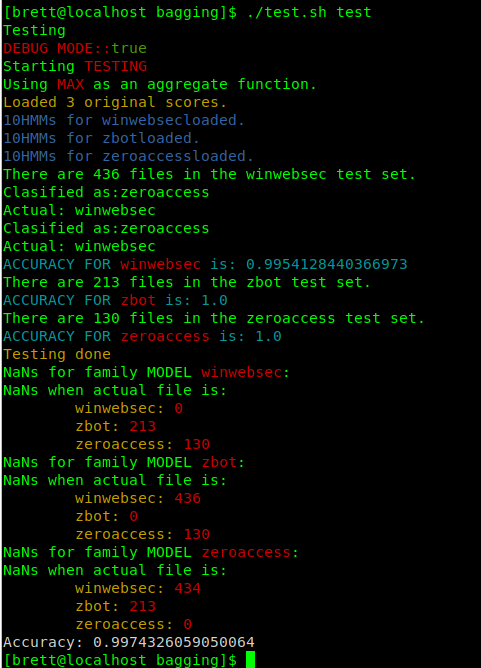
\includegraphics[width=0.5\textwidth]{bagging1.png}
          \caption{Initial results from Bagging.}
          \label{bagging1}
          \end{figure}
 

\end{document}
